% https://tex.stackexchange.com/questions/88949/curved-waved-lines-with-tikz
\documentclass[tikz]{standalone}
\usepackage[utf8]{inputenc}
\usepackage{graphicx}
\begin{document}

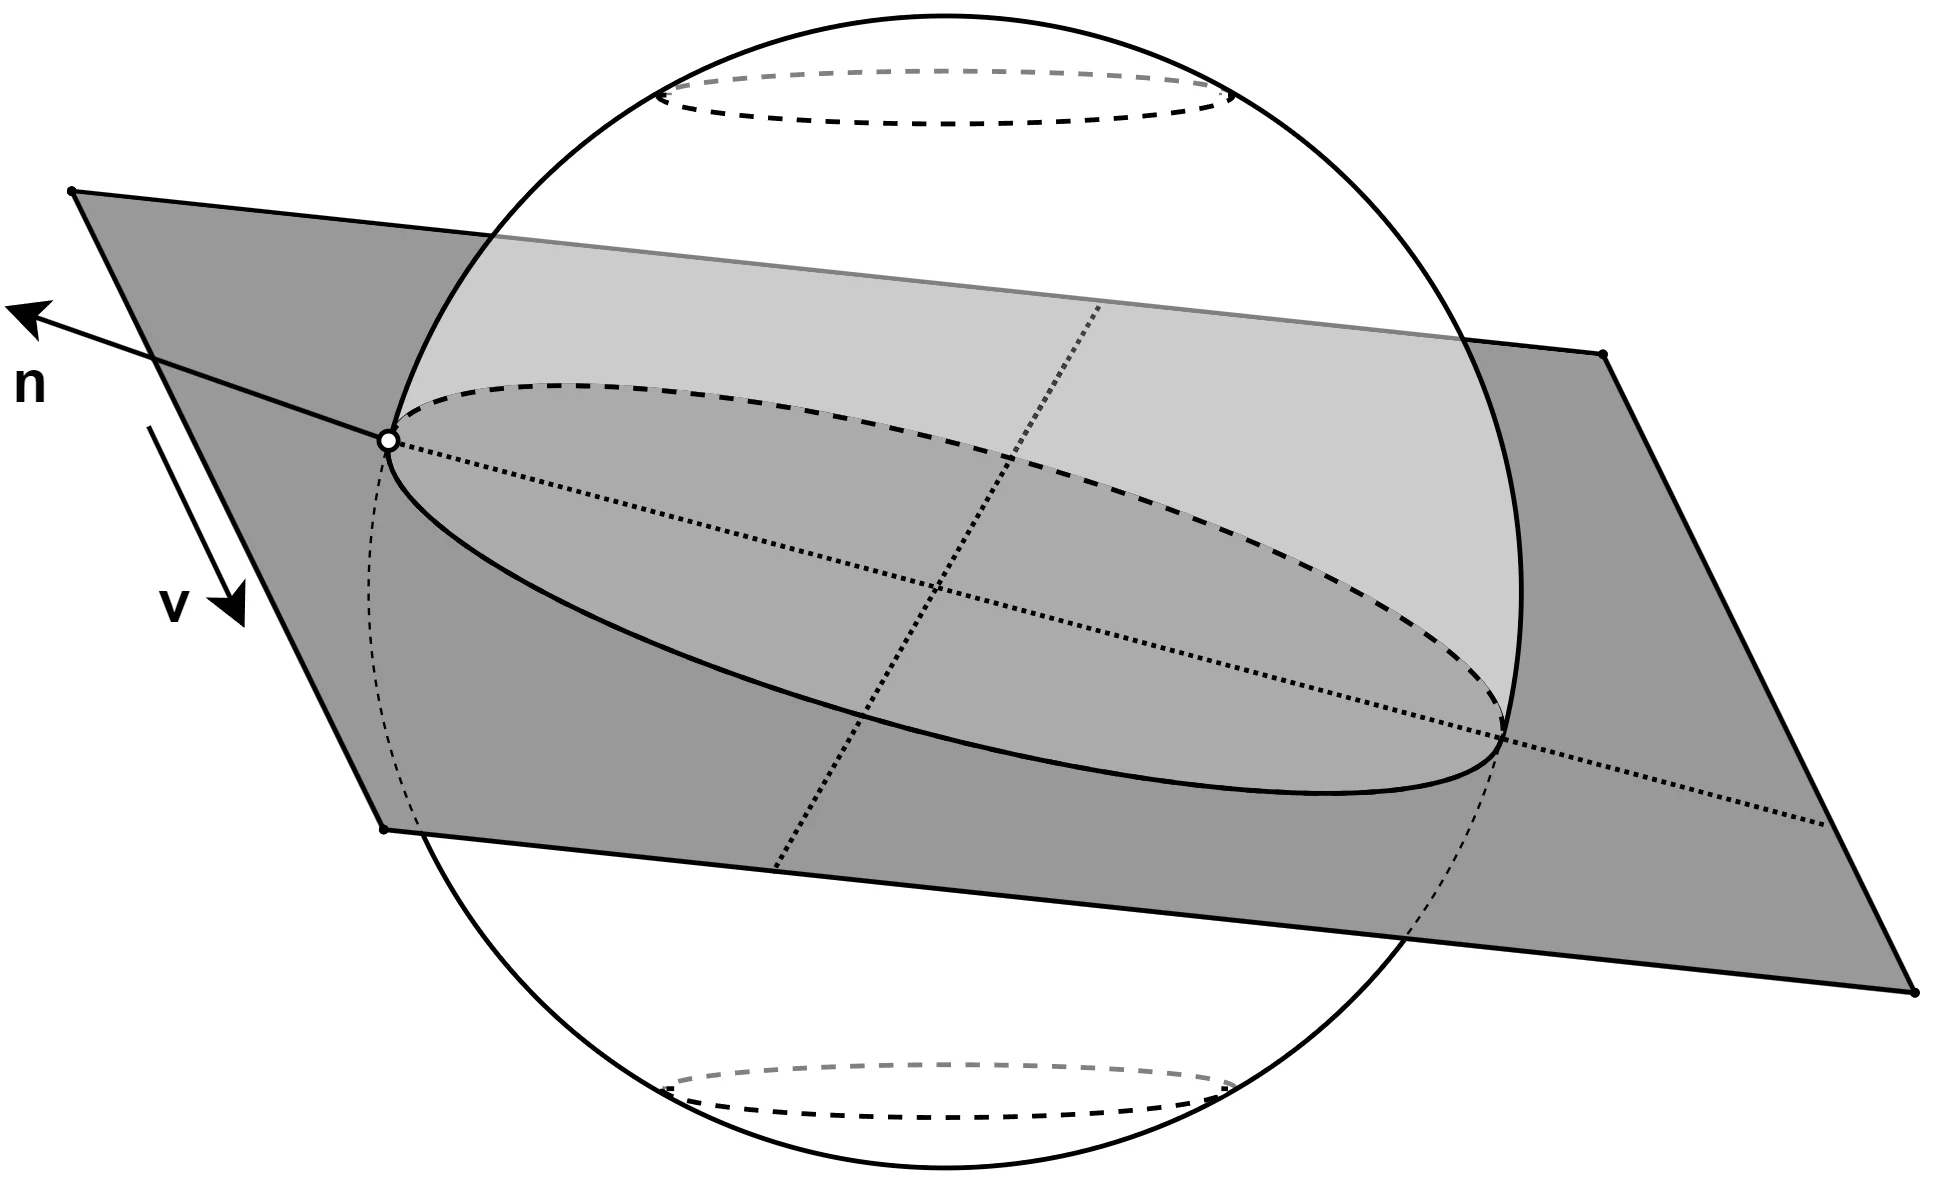
\includegraphics[width=20cm]{visuals.png}

\end{document}


\begin{tikzpicture}

\node[anchor=north west ,inner sep=0] (frame1) at (0,13)     {\includegraphics[width=20cm]{visuals-and-tools-vector-graphics-tool-recommendations-v0-1eey8pfrbicd1}};

\draw [red, very thick,] (3.9,4.35) -- (19.8,2.75) -- (16.5,9.3) -- (0.7,11) -- cycle; % fill=gray

\draw[help lines,blue] (0,0) grid (20,14);

\draw[red,thick] (9.75,6.9) circle (6cm);
\draw [red, very thick,dashed](9.75,1.75) ellipse (3cm and 0.3cm);
\draw [red, very thick,dashed](9.75,12) ellipse (3cm and 0.3cm);

 
\end{tikzpicture}